%%
\documentclass[Dissertacao, brazilian]{dissertacao-next} %%
%
% PACKAGES
%
%% Extensão de arquivo das figuras (case sensitive)
\DeclareGraphicsExtensions{.png,.jpg,.jpeg,.pdf} %
\graphicspath{ %
  %% Inclua os diretorios de figuras como o exemplo abaixo
  {./fig/} %
  {./img/} %
} %
%% ------------------------------------------------------------------------------
%%%%%%%%%%%%%%%%%%%%%%%%%%%%%%%%%%%%%%%%%%%%%%%%%%%%%%%%%%%%%%%%%%%%%%%%%%%%%%%%%%%%%%%%%%%%%%%%%%%%
%
%                                   CONFIGURAÇÂO DO PACOTE LISTINGS
%
%%%%%%%%%%%%%%%%%%%%%%%%%%%%%%%%%%%%%%%%%%%%%%%%%%%%%%%%%%%%%%%%%%%%%%%%%%%%%%%%%%%%%%%%%%%%%%%%%%%%
\usepackage{listings}
%% To handle UTF-8, you should tell listings how to interpret the special characters by defining
%% them like so

\renewcommand{\lstlistingname}{Código} %
\renewcommand{\lstlistlistingname}{Lista de \lstlistingname s} %

\lstset{ %%
  captionpos=b, % Posição da legenda
  numberbychapter=false, % Numeração das legendas por documento e não por capítulo
} %

\lstset{literate= %
  {á}{{\'a}}1 {é}{{\'e}}1 {í}{{\'i}}1 {ó}{{\'o}}1 {ú}{{\'u}}1 %
  {à}{{\`a}}1 {è}{{\`e}}1 {ì}{{\`i}}1 {ò}{{\`o}}1 {ù}{{\`u}}1 %
  {ä}{{\"a}}1 {ë}{{\"e}}1 {ï}{{\"i}}1 {ö}{{\"o}}1 {ü}{{\"u}}1 %
  {Á}{{\'A}}1 {É}{{\'E}}1 {Í}{{\'I}}1 {Ó}{{\'O}}1 {Ú}{{\'U}}1 %
  {À}{{\`A}}1 {È}{{\'E}}1 {Ì}{{\`I}}1 {Ò}{{\`O}}1 {Ù}{{\`U}}1 %
  {Ä}{{\"A}}1 {Ë}{{\"E}}1 {Ï}{{\"I}}1 {Ö}{{\"O}}1 {Ü}{{\"U}}1 %
  {â}{{\^a}}1 {ê}{{\^e}}1 {î}{{\^i}}1 {ô}{{\^o}}1 {û}{{\^u}}1 %
  {Â}{{\^A}}1 {Ê}{{\^E}}1 {Î}{{\^I}}1 {Ô}{{\^O}}1 {Û}{{\^U}}1 %
  {œ}{{\oe}}1 {Œ}{{\OE}}1 {æ}{{\ae}}1 {Æ}{{\AE}}1 {ß}{{\ss}}1 %
  %% 
  {ű}{{\H{u}}}1 {Ű}{{\H{U}}}1 {ő}{{\H{o}}}1 {Ő}{{\H{O}}}1 %
  {ç}{{\c c}}1 {Ç}{{\c C}}1 {ø}{{\o}}1 {å}{{\r a}}1 {Å}{{\r A}}1 %
  {€}{{\EUR}}1 {£}{{\pounds}}1 %
}%

%%%%%%%%%%%%%%%%%%%%%%%%%%%%%%%%%%%%%%%%%%%%%%%%%%%%%%%%%%%%%%%%%%%%%%%%%%%%%%%%%%%%%%%%%%%%%%%%%%%%
%
%%%%%%%%%%%%%%%%%%%%%%%%%%%%%%%%%%%%%%%%%%%%%%%%%%%%%%%%%%%%%%%%%%%%%%%%%%%%%%%%%%%%%%%%%%%%%%%%%%%%
\lstdefinestyle{mpasm}{%
  language=[x86masm]Assembler, %
  %basewidth={.5em,0.5em}, %
  %backgroundcolor=\color{white}, %
  breakatwhitespace=true, %
  breaklines=false, %
  extendedchars=true, %
  keepspaces=true, %
  showspaces=false, %
  showstringspaces=false, %
  showtabs=false, %
  tabsize=2, %
  xleftmargin=-10pt, %
  basicstyle=\linespread{1}\scriptsize\ttfamily, %
  keywordstyle=\color{blue}, %
  commentstyle=\color{green!40!black}, %
  stringstyle=\color{orange}, %
  %% 
  morekeywords={\#define, \#undefine, \#include, end, equ, org, processor, radix, set, constant,
  variable, if, else, ifdef, ifndef, endif, while, endw, __badram, __badrom, __maxram, __maxrom,
  __idlocks, __config, config, da, data, db, de, dt, dw, cblock, endc, fill, res, error,
  errorlevel, list, messg, nolist, page, space, subtitle, title, macro, endm, exitm, local,
  expand, noexpand, access_ovr, bankisel, banksel, code, code_pack, extern, global, idata,
  idata_acs, pagesel, pageselw, udata, udata_acs, udata_ovr, udata_shr}, %
  keywordstyle=\color{yellow!40!black}, %
  %% 
  morekeywords= {bsr, option, pcl, pch, pclath, pclatu, prodh, prodl, tblath, tblatl, tblptr,
  wreg, c, dc, z, ov,n, to, pd, gie, pc, tos, wdt, addwf, andwf, clrf, clrw, comf, decf, decfsz,
  incf, iorwf, movf, movwf, nop, rlf, rrf, subwf, swapf, xorwf, bcf, bsf, btfsc, btfss, addlw,
  andlw, call, clrwdt, goto, iorlw, movlw, option, retfie, retlw, return, sleep""sublw, tris,
  xorlw, addcf, adddcf, b, bc, bdc, bnc, bndc, bnz, bz, clrc, clrdc, clrz, lcall, lgoto, movfw,
  negf, setc, setdc, setz, skpc, skpdc, skpnc, skpndc, skpz}, %
  keywordstyle=\bfseries\color{blue}, %
} %



\lstdefinestyle{python}{%
  language=Python, %
  basewidth={.5em,0.5em}, %
  %backgroundcolor=\color{white}, %
  breakatwhitespace=true, %
  breaklines=false, %
  extendedchars=true, %
  keepspaces=true, %
  showspaces=false, %
  showstringspaces=false, %
  showtabs=false, %
  tabsize=2, %
  xleftmargin=-10pt, %
  basicstyle=\linespread{1}\scriptsize\ttfamily, %
  keywordstyle=\color{blue}, %
  commentstyle=\color{green!40!black}, %
  stringstyle=\color{purple}, %
} %



\lstdefinestyle{shell}{%
  language=bash, %
  basewidth={.5em,0.5em}, %
  %backgroundcolor=\color{white}, %
  breakatwhitespace=false, %
  breaklines=false, %
  extendedchars=false, %
  keepspaces=true, %
  showspaces=false, %
  showstringspaces=false, %
  showtabs=false, %
  tabsize=2, %
  xleftmargin=5pt, %
  basicstyle=\footnotesize\ttfamily, %
%  keywordstyle=\color{blue}, %
%  commentstyle=\color{green!40!black}, %
%  stringstyle=\color{purple}, %
%  frame=single, %
  %float=h, %
  xleftmargin=1.5cm,%
  xrightmargin=1.5cm,%
} %

\lstdefinestyle{codigoiso}{%
  basewidth={.5em,0.5em}, %
  breakatwhitespace=false, %
  breaklines=false, %
  extendedchars=false, %
  keepspaces=true, %
  showspaces=false, %
  showstringspaces=false, %
  showtabs=false, %
  tabsize=2, %
  xleftmargin=5pt, %
  basicstyle=\footnotesize\ttfamily, %
%  keywordstyle=\color{blue}, %
  commentstyle=\color{green!40!black}, %
%  stringstyle=\color{purple}, %
%  frame=single, %
  float=h, %
  %%
  morecomment=[s]{(}{)},
  %%
  morekeywords={},
} %


%%%%%%%%%%%%%%%%%%%%%%%%%%%%%%%%%%%%%%%%%%%%%%%%%%%%%%%%%%%%%%%%%%%%%%%%%%%%%%%%%%%%%%%%%%%%%%%%%%%%

\newcommand{\includempasm}[2]{\lstinputlisting[style=mpasm, fontadjust]{#1}}

\newcommand{\includepython}[2]{\lstinputlisting[style=python, fontadjust]{#1}}




%%% Local Variables:
%%% mode: latex
%%% TeX-master: "main-tcc-ifg"
%%% End:


 % Configuração
%%------------------------------------------------------------------------------
%%
%%                                      CAPA
%%
\instituicao{Universidade~Federal~de~Goiás}%
\instituicaol{Programa de Pós-Graduação em Engenharia Elétrica e da Computação}%
\instituicaosigla{[UFG] \& [EMC]}%
\instituicaocidade{Goiânia - Goiás - Brasil}%
%%
\author{Nome~do~Autor} %%
\email{email.do.autor@dominio.com} %%
%%
\titulo{Titulo da Dissertação} %%
%%
\date{\today} %%
%%
\descriccao{Dissertação apresentada à Banca Examinadora como exigência parcial para a obtenção do
  título de Mestre em Engenharia Elétrica e de Computação pela Universidade Federal de Goiás (UFG), Escola de Engenharia Elétrica, Mecânica e de Computação (EMC), sob a orientação do Prof. Dr. Wesley Pacheco Calixto e co-orientação do Prof. Dr. Fulano de Tal} %%
%%
\tituloverso{\vspace{-0.9cm}\textbf{}} %%
\descriccaoverso{} %%

% FOLHA DE ROSTO
\descriccaoversoA{} %

% FICHA CATALOGRÁFICA

\palavraschaveFICHAC{palavras-chaves,keywords}

%% 
%%                              FICHA CATALOGRÁFICA
%%

\cutterFICHAC{C1984s} %%
\autorUltimoNomeFICHAC{Sobrenome, Nome} %%
\tituloFICHAC{Titulo do Trabalho} %%
\paginasFICHAC{\pageref{LastPage} f. : il}%% número total de páginas
\cidadeFICHAC{Goiânia}%
\instituicaoFICHAC{Universidade Federal de Goiás} %
\anoFICHAC{2016}%
\palavraschaveFICHAC{%
  Orientador: Prof. Fulano de tal.\\\\
  Tese Dissertação --- Universidade Federal de Goiás.\\
  Inclui apêndices.\\\\
  1.~palvra1 --- palavra2 --- palavra3. I.~Tal, Fulano de (orientador). II.~Universidade Federal de Goiás. III.~Título.%
} %
\numeroCDDFICHAC{004.6} %% número do CDU

\FCElaboradaPor{Nome Bibliotecario CRB X/X.xxx}
\Biblioteca{Biblioteca}


%%% Local Variables:
%%% mode: latex
%%% coding: utf-8
%%% TeX-master: "main-dissertacao"
%%% End:
 % faça as modificações pertinentes no arquivo
%%------------------------------------------------------------------------------
\makeindex

%
% INICIO DO DOCUMENTO
%

\begin{document}
%%------------------------------------------------------------------------------
\maketitle
%%------------------------------------------------------------------------------
%%%%%%%%%%%%%%%%%%%%%%%%%%%%%%%%%%%%%%%%%%%%%%%%%%%%%%%%%%%%%%%%%%%%%%%%%%%%%%%%
%                                    EPÍGRAFE
%%%%%%%%%%%%%%%%%%%%%%%%%%%%%%%%%%%%%%%%%%%%%%%%%%%%%%%%%%%%%%%%%%%%%%%%%%%%%%%%

%% opcional

\begin{epigrafe} %% insira sua epígrafe abaixo; estilo livre

  \textit{\large ``Far better is it to dare mighty things, to win glorious
    triumphs, even though checkered by failure... than to rank with those poor
    spirits who neither enjoy nor suffer much, because they live in a gray
    twilight that knows not victory nor defeat.''.}

\vspace*{1cm}

\hfill%
\begin{minipage}[r]{.6\linewidth}
  \begin{center}
    \textsc{Theodore Roosevelt}\\
    \textsl{``The Man in the Arena: Citizenship in a Republic''}\\
    Paris, April 23, 1910.
  \end{center}
\end{minipage}

\end{epigrafe}

%%% Local Variables:
%%% mode: latex
%%% TeX-master: "../main-dissertacao"
%%% coding: utf-8
%%% End:
 %% opcional
%%%%%%%%%%%%%%%%%%%%%%%%%%%%%%%%%%%%%%%%%%%%%%%%%%%%%%%%%%%%%%%%%%%%%%%%%%%%%%%%
% DEDICATÓRIA
%%%%%%%%%%%%%%%%%%%%%%%%%%%%%%%%%%%%%%%%%%%%%%%%%%%%%%%%%%%%%%%%%%%%%%%%%%%%%%%% 

%% opcional

\begin{dedicatoria} %% insira sua dedicatória abaixo; estilo livre

  \newcommand{\mytext}{%
    A todas as pessoas que me apoiaram de alguma forma e tornaram possível a
    realização deste trabalho.
    % 
  }

  %% Utiliza a fonte calligra se estiver presente
  \ifcalligra
   \calligra\Large \mytext
  \else
   \itshape\Large \mytext
  \fi

\end{dedicatoria}

%%% Local Variables:
%%% mode: latex
%%% TeX-master: "../main-dissertacao"
%%% coding: utf-8
%%% End:

 %% opcional
%%%%%%%%%%%%%%%%%%%%%%%%%%%%%%%%%%%%%%%%%%%%%%%%%%%%%%%%%%%%%%%%%%%%%%%%%%%%%%%%
% AGRADECIMENTOS
%%%%%%%%%%%%%%%%%%%%%%%%%%%%%%%%%%%%%%%%%%%%%%%%%%%%%%%%%%%%%%%%%%%%%%%%%%%%%%%%

\begin{agradecimentos} %

  Agradeço a ...

  Agradeço também a ...

  Agradeço ao meu orientador ... 

\end{agradecimentos}

%%% Local Variables:
%%% mode: latex
%%% TeX-master: "../main-dissertacao"
%%% coding: utf-8
%%% End:
 %% opcional
%%%%%%%%%%%%%%%%%%%%%%%%%%%%%%%%%%%%%%%%%%%%%%%%%%%%%%%%%%%%%%%%%%%%%%%%%%%%%%%%
% RESUMO
%%%%%%%%%%%%%%%%%%%%%%%%%%%%%%%%%%%%%%%%%%%%%%%%%%%%%%%%%%%%%%%%%%%%%%%%%%%%%%%%

\begin{resumo}

  Este trabalho ...

\end{resumo}

%%% Local Variables:
%%% mode: latex
%%% TeX-master: "../main-dissertacao"
%%% coding: utf-8
%%% End:
 %% obrigatório
%%%%%%%%%%%%%%%%%%%%%%%%%%%%%%%%%%%%%%%%%%%%%%%%%%%%%%%%%%%%%%%%%%%%%%%%%%%%%%%%
% ABSTRACT
%%%%%%%%%%%%%%%%%%%%%%%%%%%%%%%%%%%%%%%%%%%%%%%%%%%%%%%%%%%%%%%%%%%%%%%%%%%%%%%%

\begin{abstract}

  This work ...
  
\end{abstract}

%%% Local Variables:
%%% mode: latex
%%% TeX-master: "../main-dissertacao"
%%% coding: utf-8
%%% End:

 %% obrigatório
%%------------------------------------------------------------------------------
\includeSumario % obrigatório, gerado automaticamente
\includeListaFiguras % obrigatório caso haja mais de 3 figuras
\includeListaTabelas % obrigatório caso haja mais de 3 tabelas
%%------------------------------------------------------------------------------
%%%%%%%%%%%%%%%%%%%%%%%%%%%%%%%%%%%%%%%%%%%%%%%%%%%%%%%%%%%%%%%%%%%%%%%%%%%%%%%%
% SIGLAS E ABREVIATURAS
%%%%%%%%%%%%%%%%%%%%%%%%%%%%%%%%%%%%%%%%%%%%%%%%%%%%%%%%%%%%%%%%%%%%%%%%%%%%%%%%

% sigla (separador: &--&) significado (quebra de linha: \\)

\begin{abreviaturasesiglas}%

  SIGLA &--& Sigla \\

  % Saltar uma linha entra cada sigla

\end{abreviaturasesiglas}

%%% Local Variables:
%%% mode: latex
%%% TeX-master: "../main-dissertacao"
%%% coding: utf-8
%%% End:

%%------------------------------------------------------------------------------
\inicioIntroducao %%
%%------------------------------------------------------------------------------
%%%%%%%%%%%%%%%%%%%%%%%%%%%%%%%%%%%%%%%%%%%%%%%%%%%%%%%%%%%%%%%%%%%%%%%%%%%%%%%%
% CAPÍTULO 1
%%%%%%%%%%%%%%%%%%%%%%%%%%%%%%%%%%%%%%%%%%%%%%%%%%%%%%%%%%%%%%%%%%%%%%%%%%%%%%%%

\chapter{Introdução} %
\label{chap:introducao} %




%%% Local Variables:
%%% mode: latex
%%% TeX-master: "../main-dissertacao"
%%% coding: utf-8
%%% End:
 %% Introdução
%%%%%%%%%%%%%%%%%%%%%%%%%%%%%%%%%%%%%%%%%%%%%%%%%%%%%%%%%%%%%%%%%%%%%%%%%%%%%%%%
% CAPÍTULO 2
%%%%%%%%%%%%%%%%%%%%%%%%%%%%%%%%%%%%%%%%%%%%%%%%%%%%%%%%%%%%%%%%%%%%%%%%%%%%%%%%

\chapter{Título do capítulo}
\label{cap:capitulo-2}

Neste Capítulo ...

Acabei de colocar aqui uma figura que é a marca do NExT, veja-a Fig.~\ref{fig:next}.

\begin{figure}[h!]
  \begin{center}
    
\includegraphics[width=5cm]{next}
    \caption{Marca do NExT.}
    \label{fig:next}
  \end{center}
\end{figure}

Assim é que colocamos as figuras:

\begin{figure}[h!]
  \begin{center}
    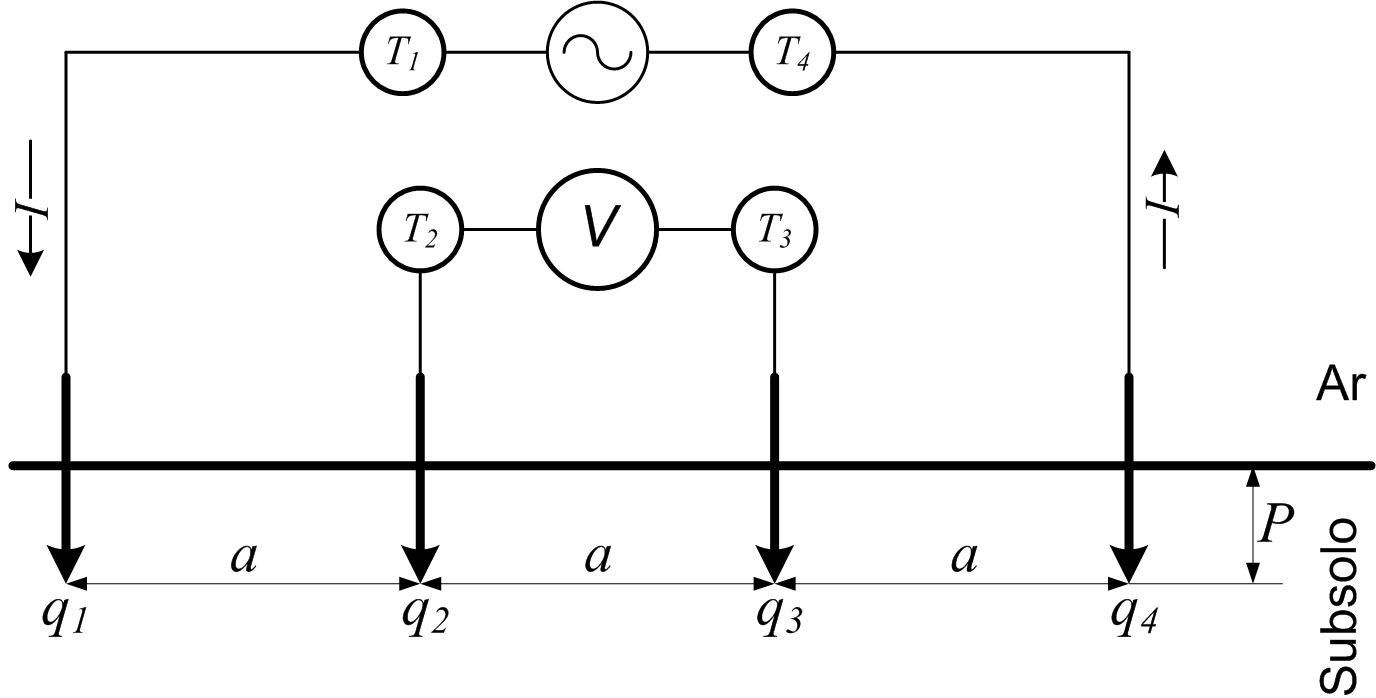
\includegraphics[width=.6\textwidth]{fig21}
    \caption{Método de \index{Wenner} Wenner.}
    \label{fig:metodo-wener}
  \end{center}
\end{figure}



Assim é que colocamos as equações:

\begin{equation}
  V_{q2} = \frac{\rho \cdot I}{4\pi}\left[\frac{1}{a} + \frac{1}{\sqrt{a^2 + (2P)^2}} - \frac{1}{2a} - \frac{1}{\sqrt{(2a)^2 + (2P)^2}}\right]
  \label{eq21}
\end{equation}

\begin{equation}
  V_{q3} = \frac{\rho \cdot I}{4\pi}\left[\frac{1}{2a} + \frac{1}{\sqrt{(2a)^2 + (2P)^2}} - \frac{1}{a} - \frac{1}{\sqrt{a^2 + (2P)^2}}\right]
  \label{eq22}
\end{equation}

Em (\ref{eq21}) e (\ref{eq22}), $a$ é a distância entre os \index{eletrodos} eletrodos, $P$ é a profundidade do eletrodo, $\rho$ a resistividade do solo. A diferença de potencial entre os pontos $q_2$ e $q_3$ é dada pela expressão (\ref{eq23}).

\begin{equation}
  V=V_{q2} - V_{q3} = \frac{\rho \cdot I}{4\pi}\left[\frac{1}{a} + \frac{1}{\sqrt{a^2 + (2P)^2}} - \frac{1}{\sqrt{(2a)^2 + (2P)^2}}\right]
  \label{eq23}
\end{equation}

Dividindo-se a diferença de potencial (\ref{eq23}) pela corrente $I$, obtém-se uma grandeza $R_m$ dimensionalmente igual a uma resistência elétrica \cite{bb14}.

\begin{equation}
  R_m = \frac{\rho}{4\pi}\left[\frac{1}{a} + \frac{1}{\sqrt{a^2 + 4P^2}} - \frac{1}{\sqrt{4a^2 + 4P^2}}\right]
  \label{eq24}
\end{equation}

Logo, isolando $\rho$ em (\ref{eq24}), tem-se a expressão para o cálculo da resistividade elétrica do solo.

\begin{equation}
  \rho = \frac{4 \pi a R_m}{1 + \frac{2a}{\sqrt{a^2 + 4P^2}} - \frac{2a}{\sqrt{4a^2 + 4P^2}}}
  \label{eq25}
\end{equation}

Para cada distância $a$ têm-se os valores de $V$ e $I$, medidos em campo e consequentemente obtém-se $R_m$ e, portanto pode-se calcular $\rho$ em (\ref{eq25}). Como o solo foi inicialmente considerado homogêneo, variando-se $a$, o valor de $R_m$ deve também variar de tal forma que $\rho$ permanece inalterado em (\ref{eq25}). Porém, na prática, o solo dificilmente se comporta com \index{homogeneidade} homogeneidade, e assim, o valor de $\rho$ calculado em (\ref{eq25}) deve variar com a distância $a$. A grandeza $\rho$ deixa de ter o significado de resistividade elétrica do solo, porém, contêm nos seus valores em função de $a$, propriedades que permitem identificar as diversas camadas homogêneas do solo.



%%% Local Variables:
%%% mode: latex
%%% TeX-master: "../main-dissertacao"
%%% coding: utf-8
%%% End:
 %% 
%%%%%%%%%%%%%%%%%%%%%%%%%%%%%%%%%%%%%%%%%%%%%%%%%%%%%%%%%%%%%%%%%%%%%%%%%%%%%%%%
% CAPÍTULO 3
%%%%%%%%%%%%%%%%%%%%%%%%%%%%%%%%%%%%%%%%%%%%%%%%%%%%%%%%%%%%%%%%%%%%%%%%%%%%%%%%


\chapter{Modelagem Matemática}

Neste Capítulo é apresentada...



%%% Local Variables:
%%% mode: latex
%%% TeX-master: "../main-dissertacao"
%%% coding: utf-8
%%% End:





 %% 
%%%%%%%%%%%%%%%%%%%%%%%%%%%%%%%%%%%%%%%%%%%%%%%%%%%%%%%%%%%%%%%%%%%%%%%%%%%%%%%%
% CAPÍTULO 4
%%%%%%%%%%%%%%%%%%%%%%%%%%%%%%%%%%%%%%%%%%%%%%%%%%%%%%%%%%%%%%%%%%%%%%%%%%%%%%%%


\chapter{Procedimentos e Metodologia}
\label{cap:metodologia}

Assim é que colocamos uma tabela:

\begin{table}[h!]
\renewcommand{\arraystretch}{1.3}
\caption{Manipulação dos dados medidos para a produção da curva $\rho_{aE}(a)$.}
\centering
\begin{tabular}{c||c||c||c||c||c||c||c||c}\hline
\bfseries $\rho_a(a)$ & \bfseries $D_1$ & \bfseries $D_2$ & \bfseries $D_3$ & \bfseries $D_4$ & \bfseries $D_5$ & \bfseries $D_6$ & \bfseries $D_7$ & \bfseries Média \\\hline\hline
$\rho_a(1)$  & $11487$ & $12615$ & $11538$ & $11929$ & $11561$ & $11642$ & $13084$ & $11979$\\
$\rho_a(2)$  & $10032$ & $9901$  & $9922$  & $9982$  & $9881$  & $10027$ & $9873$  & $9945$ \\
$\rho_a(4)$  & $7781$  & $8009$  & $7979$  & $8179$  & $8194$  & $7878$  & $8301$  & $8046$ \\
$\rho_a(8)$  & $14820$ & $14424$ & $14460$ & $14297$ & $14246$ & $14209$ & $14011$ & $14352$\\
$\rho_a(16)$ & $14931$ & $15693$ & $16397$ & $15451$ & $15825$ & $15273$ & $16459$ & $15718$\\
$\rho_a(32)$ & $10334$ & $9138$  & $9046$  & $9599$  & $10148$ & $8991$  & $20187$ & $11063$\\\hline
\end{tabular}
\label{tab41new}
\end{table}

Você também pode utilizar o Software La Table para gerar tabela e colocá-la no \LaTeX, conforme \cite{bb20}. Conforme a expressão (\ref{eq00})

\begin{equation}
 F(x) = \sum_{-\infty}^{+\infty} \xi \cdot \sum_{-\infty}^{+\infty} \gamma
 \label{eq00}
\end{equation}



\begin{table}[h!]
\renewcommand{\arraystretch}{1.3}
\caption{Teste da primeira aula em \LaTeX, veja Fig.~\ref{fig:metodo-wener}.}
\centering
\begin{tabular}{c|||c|||c||c||c||c||c||c||c}\hline
\bfseries $\rho_a(a)$ & \bfseries $D_1$ & \bfseries $D_2$ & \bfseries $D_3$ & \bfseries $D_4$ & \bfseries $D_5$ & \bfseries $D_6$ & \bfseries $D_7$ & \bfseries Média \\\hline\hline
$\rho_a(1)$  & $11487$ & $12615$ & $11538$ & $11929$ & $11561$ & $11642$ & $13084$ & $11979$\\
$\rho_a(2)$  & $10032$ & $9901$  & $9922$  & $9982$  & $9881$  & $10027$ & $9873$  & $9945$ \\\hline
$\rho_a(4)$  & $7781$  & $8009$  & $7979$  & $8179$  & $8194$  & $7878$  & $8301$  & $8046$ \\
$\rho_a(8)$  & $14820$ & $14424$ & $14460$ & $14297$ & $14246$ & $14209$ & $14011$ & $14352$\\\hline\hline
$\rho_a(16)$ & $14931$ & $15693$ & $16397$ & $15451$ & $15825$ & $15273$ & $16459$ & $15718$\\
$\rho_a(32)$ & $10334$ & $9138$  & $9046$  & $9599$  & $10148$ & $8991$  & $20187$ & $11063$\\\hline
\end{tabular}
\label{tab41new}
\end{table}


%\begin{tabular}{lll|l}
%\hline
%\multicolumn{2}{c|}{Janela} & \multicolumn{2}{c|}{Porta} \\
%\hline
%\multicolumn{1}{l|}{1} & \multicolumn{1}{l|}{2} & 3 & 4 \\
%\hline
%\multicolumn{4}{c|}{Casa} \\
%\hline
%\multicolumn{1}{l|}{a} & \multicolumn{2}{c|}{ab} & b \\
%\hline
%\multicolumn{1}{l|}{c} & \multicolumn{1}{l|}{d} & f & g \\
%\hline
%\end{tabular}


%%% Local Variables:
%%% mode: latex
%%% TeX-master: "../main-dissertacao"
%%% coding: utf-8
%%% End:
 %% 
% E assim por diante até a conclusão
%%%%%%%%%%%%%%%%%%%%%%%%%%%%%%%%%%%%%%%%%%%%%%%%%%%%%%%%%%%%%%%%%%%%%%%%%%%%%%%%
% CAPÍTULO XX
%%%%%%%%%%%%%%%%%%%%%%%%%%%%%%%%%%%%%%%%%%%%%%%%%%%%%%%%%%%%%%%%%%%%%%%%%%%%%%%%

\chapter{Conclusão} %
\label{chap:canclusao} %


Durante todo o percurso para o término deste trabalho... 

\section{Contribuições do Trabalho}
As contribuições podem assim ser descritas:


\textbf{Artigos em revista:}

\textbf{Artigos em congresso:}

\textbf{Patentes e Registros:}

\section{Sugestões para Trabalhos Futuros}






%%% Local Variables:
%%% mode: latex
%%% TeX-master: "../main-dissertacao"
%%% coding: utf-8
%%% End:

%%------------------------------------------------------------------------------
\bibliographystyle{abntex2-alf}%
\bibliography{referencias}%
%%------------------------------------------------------------------------------
\inicioAnexo
%%%%%%%%%%%%%%%%%%%%%%%%%%%%%%%%%%%%%%%%%%%%%%%%%%%%%%%%%%%%%%%%%%%%%%%%%%%%%%%%
% ANEXO 1
%%%%%%%%%%%%%%%%%%%%%%%%%%%%%%%%%%%%%%%%%%%%%%%%%%%%%%%%%%%%%%%%%%%%%%%%%%%%%%%%

\chapter{Título do Anexo}
\label{cap:anexo1}

Abaixo o desenvolvimento do...

%%% Local Variables:
%%% mode: latex
%%% TeX-master: "../main-dissertacao"
%%% coding: utf-8
%%% End:




 %%
%%------------------------------------------------------------------------------

\inicioApendice %
%%%%%%%%%%%%%%%%%%%%%%%%%%%%%%%%%%%%%%%%%%%%%%%%%%%%%%%%%%%%%%%%%%%%%%%%%%%%%%%%
% APENDICES
%%%%%%%%%%%%%%%%%%%%%%%%%%%%%%%%%%%%%%%%%%%%%%%%%%%%%%%%%%%%%%%%%%%%%%%%%%%%%%%%

\chapter{Título do apêndice}
\label{chap:apendice-chap-1}

Neste Apêndice ...


\section{Exemplo de código fonte}
\label{chap:codigo-fonte}

Abaixo está o código fonte ...

Para incluir um codigo fonte, edite as configuracoes do arquivo \textbf{config-listings.tex}.

%% \includempasm{<caminho-do-arquivo.asm>}{nome-do-codigo}

%%% Local Variables:
%%% mode: latex
%%% TeX-master: "../main-dissertacao"
%%% coding: utf-8
%%% End:
 %%

%%------------------------------------------------------------------------------
%% %%%%%%%%%%%%%%%%%%%%%%%%%%%%%%%%%%%%%%%%%%%%%%%%%%%%%% 
% Glossário
%%%%%%%%%%%%%%%%%%%%%%%%%%%%%%%%%%%%%%%%%%%%%%%%%%%%%% 

\begin{glossario}
  \label{glossario}

\item[Condutivímetro] - é um medidor digital portátil que mensura a condutividade elétrica do solo diretamente "\emph{in loco}".

\item[Data Logger] - é um coletor de dados também chamado de datalogger ou gravador de dados. É um dispositivo eletrônico que registra os dados ao longo do tempo ou em relação a uma localização, construído com sensores externos. São baseados em um processador digital com memórias internas para armazenamento de dados. São de uso geral para uma gama de aplicações em dispositivos de medição específicos, podem ser programáveis.

\item[GPS] - é um sistema de navegação por satélite que fornece a um aparelho receptor móvel a posição do mesmo, assim como informação horária, sob todas quaisquer condições atmosféricas, a qualquer momento e em qualquer lugar na Terra, desde que o receptor se encontre no campo de visão de quatro satélites GPS.

\item[Neossolo Regolítico] - são tipos de solos que apresentam textura arenosa e baixa capacidade de adsorção de nutrientes, quando comparado com solos argilosos, possui baixo teor de matéria orgânica e nitrogênio que diminuem, após alguns anos de uso agrícola.

\item[Nitossolo Vermelho] - são solos minerais, não-hidromórficos, apresentando cor vermelho-escura tendendo à arroxeada. São derivados do intemperismo de rochas básicas e ultrabásicas, ricas em minerais ferromagnesianos. Uma característica peculiar é que esses solos, como os Latossolos Roxos, apresentam materiais que são atraídos pelo imã. Seus teores de ferro ($Fe2O3$) são elevados (superiores a 15\%).

\item[Plintossolo Pétrico Concrecionário] - são solos que ocorrem em áreas baixas e nas bordas das chapadas, constituindo geralmente por solos pobres em nutrientes. A origem de concreções ferruginosas nos solos tem sido atribuída, de forma generalizada, às condições de variações sazonais do lençol freático. Este, inicialmente elevado, propicia a redução do ferro com a sua retirada parcial do sistema, mobilização, transporte e concentração. Posteriormente, em épocas secas, a oxidação forma plintitas constituídas por mistura de argila pobre em \emph{C} orgânico e rica em ferro e alumínio, segregada sob a forma de manchas vermelhas, que com a retirada do lençol freático, apresentam endurecimento constituindo concreções ferruginosas ou petroplintitas.

\item[PVC] - é feito a partir de repetidos processos de polimerização que convertem hidrocarbonetos, contidos em materiais como o petróleo, em um único composto chamado polímero. O vinil é formado basicamente por etileno e cloro. Por uma reação química, o etileno e o cloro combinam-se formando o dicloreto de etileno, que por sua vez é transformado em um gás chamado \emph{VCM} (Vinyl chloride monomer, em português cloreto de vinila). O passo final é a polimerização, que converte o monómero num polímero de vinil, que é o \emph{PVC}, ou simplesmente vinil, contém, em peso, $57\%$ de cloro (derivado do cloreto de sódio - sal de cozinha) e $43\%$ de eteno (derivado do petróleo).

\item[TC scan] - é uma tomografia computadorizada (\emph{TC}), originalmente apelidada tomografia axial computadorizada (\emph{TAC}), é um exame complementar de diagnóstico por imagens tridimensionais, que consiste numa representação de uma secção ou fatia do estudo. É obtida através do processamento por computador de informação recolhida após expor o objeto estudado a uma sucessão de raios $X$. Seu método principal é estudar a atenuação de um feixe de raios $X$ durante seu trajeto através de um segmento do objeto estudado; no entanto, ela se distingue da radiografia convencional em diversos elementos.

\end{glossario}

%%% Local Variables:
%%% mode: latex
%%% TeX-master: "../main-dissertacao"
%%% coding: utf-8
%%% End:

%%------------------------------------------------------------------------------
\inicioIndice %
%%------------------------------------------------------------------------------
\end{document}

%
% FIM DO DOCUMENTO
%

%%% Local Variables:
%%% mode: latex
%%% TeX-master: t
%%% coding: utf-8
%%% End:
